\documentclass[preview]{standalone}

\usepackage{amsmath}
\usepackage{amssymb}
\usepackage{bettelini}
\usepackage{stellar}
\usepackage{definitions}

\newcommand{\baseframe}{
    \draw[->] (-0.03,0) -- (1.08,0) node[right] {$x$};
    \draw[thin] (0,0) rectangle (1,1);
    \node[below left] at (0,0) {$0$};
    \node[below] at (1,0) {$1$};
    \node[left] at (0,1) {$1$};
}

\begin{document}

\id{measuretheory-cantor-function}
\genpage

\section{The Cantor Function}

\begin{snippetdefinition}{cantor-vitali-function-definition}{Cantor--Vitali function}
    Define \(F_0\colon[0,1]\fromto[0,1]\) by \(F_0(x)=x\). Recursively, let
    \[
        F_{n+1}(x)=
        \begin{cases}
            \dfrac12F_n(3x),
                &x\in\left[0,\dfrac13\right],\\[1.2em]
            \dfrac12,
                &x\in\left[\dfrac13,\dfrac23\right],\\[1.2em]
            \dfrac12+\dfrac12F_n(3x-2),
                &x\in\left[\dfrac23,1\right].
        \end{cases}
    \]
    The sequence \(F_n\) converges uniformly on \([0,1]\). Its limit
    \[
        F(x)=\lim_{n\to\infty}F_n(x)
    \]
    is called the \emph{Cantor--Vitali function}, or the
    \emph{devil's staircase}.
\end{snippetdefinition}

\begin{snippet}{cantor-vitali-function-approximations}
    \begin{center}
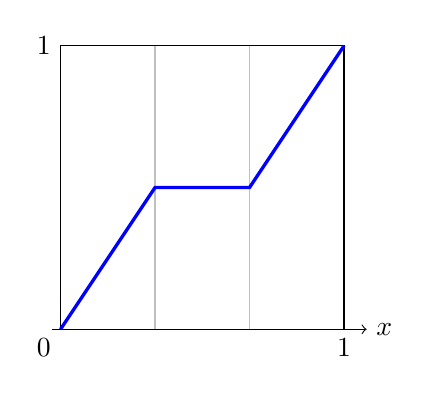
\begin{tikzpicture}[scale=0.9,x=4cm,y=4cm,baseline=(current bounding box.center)]
        \baseframe
        \draw[gray!50, thin] (1/3,0) -- (1/3,1);
        \draw[gray!50, thin] (2/3,0) -- (2/3,1);
        \draw[blue, very thick]
        (0,0) --
        (1/3,1/2) --
        (2/3,1/2) --
        (1,1);
    \end{tikzpicture}
        \hspace{0.4cm}
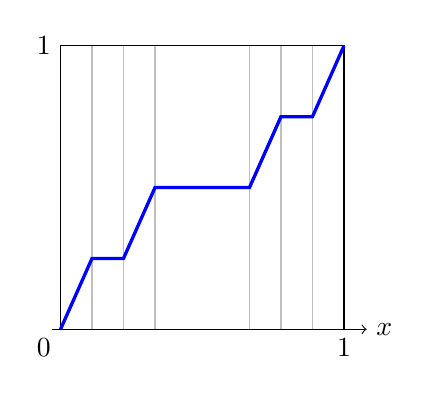
\begin{tikzpicture}[scale=0.9,x=4cm,y=4cm,baseline=(current bounding box.center)]
        \baseframe
        \foreach \x in {1/9,2/9,1/3,2/3,7/9,8/9}
        \draw[gray!50, thin] (\x,0) -- (\x,1);
        \draw[blue, very thick]
        (0,0) --
        (1/9,1/4) --
        (2/9,1/4) --
        (1/3,1/2) --
        (2/3,1/2) --
        (7/9,3/4) --
        (8/9,3/4) --
        (1,1);
    \end{tikzpicture}
        \hspace{0.4cm}
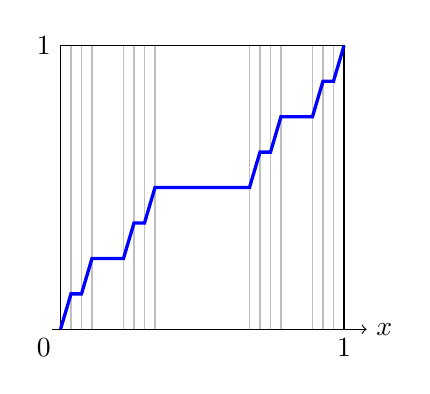
\begin{tikzpicture}[scale=0.9,x=4cm,y=4cm,baseline=(current bounding box.center)]
        \baseframe
        \foreach \x in {1/27,2/27,1/9,2/9,7/27,8/27,1/3,2/3,19/27,20/27,7/9,8/9,25/27,26/27}
        \draw[gray!50, thin] (\x,0) -- (\x,1);
        \draw[blue, very thick]
        (0,0) --
        (1/27,1/8) --
        (2/27,1/8) --
        (1/9,1/4) --
        (2/9,1/4) --
        (7/27,3/8) --
        (8/27,3/8) --
        (1/3,1/2) --
        (2/3,1/2) --
        (19/27,5/8) --
        (20/27,5/8) --
        (7/9,3/4) --
        (8/9,3/4) --
        (25/27,7/8) --
        (26/27,7/8) --
        (1,1);
    \end{tikzpicture}
    \end{center}
\end{snippet}

\begin{snippettheorem}{cantor-vitali-function-properties}{Properties of the Cantor function}
    The Cantor--Vitali function \(F\) is continuous, nondecreasing and
    surjective from \([0,1]\) to \([0,1]\). It is locally constant on the
    complement of the Cantor set. Consequently,
    \[
        F'(x)=0
    \]
    almost everywhere, but \(F(1)-F(0)=1\).
\end{snippettheorem}

\begin{snippet}{cantor-function-not-recovered-from-derivative}
    The Cantor function shows that almost-everywhere differentiability and an
    integrable derivative do not suffice for
    \[
        f(x)=f(0)+\int_0^xf'(t)\,dt.
    \]
    Indeed, its derivative is zero almost everywhere while the function is
    not constant.
\end{snippet}

\begin{snippettheorem}{absolute-continuity-fundamental-theorem-characterization}{Absolute continuity and recovery from the derivative}
    Let \(f\colon[a,b]\fromto\realnumbers\). The function \(f\) is absolutely
    continuous if and only if there exists \(g\in L^1([a,b])\) such that
    \[
        f(x)=f(a)+\int_a^xg(t)\,dt
    \]
    for every \(x\in[a,b]\). In this case \(f'=g\) almost everywhere, and
    therefore
    \[
        f(x)=f(a)+\int_a^xf'(t)\,dt.
    \]
\end{snippettheorem}

\begin{snippetcorollary}{cantor-function-not-absolutely-continuous}{The Cantor function is not absolutely continuous}
    The Cantor--Vitali function is continuous and differentiable almost
    everywhere, but it is not absolutely continuous.
\end{snippetcorollary}

\section{Composition of Measurable Functions}

\begin{snippetexample}{composition-lebesgue-measurable-functions-not-measurable}{A composition of Lebesgue measurable functions need not be measurable}
    Let \(F\) be the Cantor function and define
    \[
        g(x)=x+F(x),
        \qquad g\colon[0,1]\fromto[0,2].
    \]
    The map \(g\) is strictly increasing and continuous, hence a homeomorphism
    onto \([0,2]\). Let \(C\) be the Cantor set and
    \(A=[0,1]\setminus C\). The set \(A\) is the disjoint union of the open
    middle thirds \(I_k\). Since \(F\) is constant on each \(I_k\), the map
    \(g\) acts there as a translation. Therefore
    \[
        \mu(g(A))
        =\sum_k\mu(g(I_k))
        =\sum_k\mu(I_k)
        =1.
    \]
    Since \([0,2]=g(A)\sqcup g(C)\), it follows that \(\mu(g(C))=1\).

    Choose a nonmeasurable set \(D\subseteq g(C)\), and let
    \(B=g^{-1}(D)\subseteq C\). The set \(B\) is Lebesgue measurable because
    it is contained in the null set \(C\), although it is not Borel. Hence
    \(\chi_B\) is Lebesgue measurable and \(g^{-1}\) is continuous, but
    \[
        \chi_B\circ g^{-1}=\chi_D
    \]
    is not Lebesgue measurable. Thus composing two Lebesgue measurable maps
    need not preserve measurability, even when the inner map is continuous.
\end{snippetexample}

\end{document}
